% Indicate the main file. Must go at the beginning of the file.
% !TEX root = ../main.tex

%----------------------------------------------------------------------------------------
% CHAPTER TEMPLATE
%----------------------------------------------------------------------------------------


\chapter{Erste Experimente und Evaluierung} % Main chapter title

\label{Chapter4} % Change X to a consecutive number; for referencing this chapter elsewhere, use \ref{ChapterX}

%----------------------------------------------------------------------------------------
% SECTION 1
%----------------------------------------------------------------------------------------
\section{Erstes Experiment mit der Churn-Metrik}
In der Literatur finden sich unterschiedliche Aussagen zum Einfluss der Code-Grösse auf die Dauer von Pull Requests (PR Latency). Während einige Studien einen klaren Zusammenhang feststellen, bleiben andere Untersuchungen uneindeutig \parencite{hasan_understanding_2023}\parencite{kudrjavets_small_2022}.

Hierfür entwickelten wir das Jupyter Notebook \textit{churn-analysis} \parencite{stumpf_simon_repo-detectivesba-metric-analysis-scripts_nodate}. Das Notebook importiert automatisiert sämtliche Repository-Daten aus den Projektmodulen des PM2-Moduls der Klassen IT21tb (Teilzeit, 2021) und IT23a (Vollzeit, 2023). Anschliessend werden die Daten durch das Mining aufbereitet und in einer Analyse zusammengeführt.

Die zentralen Schritte der Analyse beinhalten:

\begin{itemize}
    \item Das Einlesen und Parsen der Pull Request Daten aller Studierenden-Projekte.
    \item Die Berechnung des Churn-Werts pro Pull Request, welcher sich aus den summierten Codezeilen-Änderungen ergibt (Additionen + Löschungen).
    \item Die Korrelation der Churn-Werte mit der gemessenen Pull Request Dauer (\textit{latency}).
    \item Das Visualisieren dieser Zusammenhänge mittels Scatterplots und Regressionslinien.
\end{itemize}

Das Ziel dieses Experiments war es, zu prüfen, ob ein signifikanter Zusammenhang zwischen der Menge an geändertem Code (Churn) und der PR-Latenz besteht.

\subsection{Outliers}
Damit keine Outliers die Datenanalyse beeinflussen, wurden diese vorgängig entfernt. Sämtliche Outliers (insegsamt 3 PRs) gehörten alle zum gleichen Projekt. Diese Pull Requests umfassen jeweils über \textit{100'000} Änderungen. 

\subsection{Ergebnisse der Churn-Analyse}

Die initiale Auswertung zeigte, dass der durchschnittliche Churn-Wert in den PM2-Projekten deutlich variiert. Einzelne Pull Requests wiesen einen sehr hohen Churn auf (über 1000 Zeilen geändert), während viele Änderungen im Bereich von 10 bis 50 Zeilen lagen. 

Die Datenanalyse ergab folgende Erkenntnisse:

\begin{itemize}
    \item \textbf{Korrelation:} Es konnte eine schwache positive Korrelation zwischen dem Churn und der PR-Latenz festgestellt werden. Grössere Pull Requests hatten tendenziell eine längere Review- und Merge-Dauer.
    \item \textbf{Ausreisser:} Besonders umfangreiche Pull Requests führten teilweise zu aussergewöhnlich langen Latenzzeiten, was sich als typische Herausforderung im Code Review Prozess darstellt.
    \item \textbf{Review-Aktivität:} Pull Requests mit geringem Churn wurden häufig schneller bearbeitet, was die Hypothese unterstützt, dass kleinere Changes leichter zu prüfen sind.
    \item \textbf{Kein Unterschied zwischen den Klassen:} Es lässt sich kein wesentlicher Unterschied zwischen der Teilzeit- und der Vollzeitklasse feststellen.
\end{itemize}

Die Ergebnisse der Scatterplots verdeutlichen diese Tendenzen. In Abbildung \ref{fig:pr-latency-churn-added-plus-deleting} ist die Korrelation grafisch dargestellt.


\begin{figure}[th]
\centering
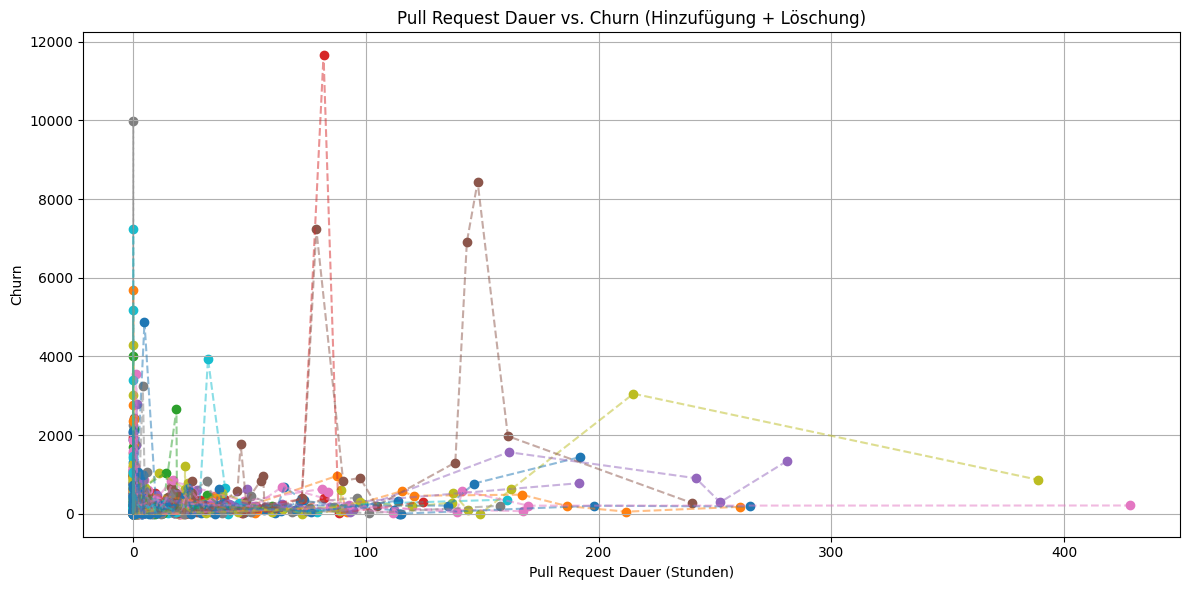
\includegraphics[width=\textwidth]{Figures/pr-latency-churn.png}
\decoRule
\caption{Scatterplot der Churn-Werte in Relation zur PR-Latenz}
\label{fig:pr-latency-churn-added-plus-deleting}
\end{figure}


Zusammenfassend liefert das erste Experiment Hinweise darauf, dass ein erhöhter Churn tatsächlich mit einer höheren PR-Latenz einhergeht. Um diese Hypothese jedoch weiter zu festigen, sind weitere Analysen und statistische Tests notwendig, die im nächsten Kapitel beschrieben werden.

%-----------------------------------
% SUBSECTION 2 (optional)
%-----------------------------------

\subsection{Fazit des ersten Experiments}

Das Experiment zur Churn-Metrik bildete die Grundlage für unsere weiteren Analysen. Es zeigte sich, dass in den studentischen Projekten ähnliche Muster auftreten wie in professionellen Softwareentwicklungsprozessen, was die Relevanz und Generalisierbarkeit der Untersuchung unterstreicht.